% Chapter Template

\chapter{Temporal Coherent Backmapping of Molecular Trajectories} % Main chapter title
\label{temp_coherent_bm} % Change X to a consecutive number; for referencing this chapter elsewhere, use \ref{ChapterX}

MD simulations evolve a molecular system in time and produce a trajectory, i.e. a discretized path in phase space. Typically, consecutive frames of the trajectory are separated by a fixed time step, which controls the correlation between recorded frames. Computing time averages over a trajectory yields structural or thermodynamic properties, such as the radial distribution function or energies. However, temporal information stored in the trajectory can be used to compute dynamic properties as well. In particular, time correlations can be used to link simulation results to experimental observables. Examples include (1) the diffusion constant, which can be computed as the integral of the velocity auto-correlation \cite{frenkel2001understanding}, (2) (infrared) absorption spectra, which are related to the auto-correlation function of the total dipole moment \cite{bergsma1984electronic, guillot1991molecular}, and (3) scattering functions that can be related to Fourier transforms of the van Hove correlation function, which is a time-dependent pair correlation function \cite{PhysRevE.53.2382, moe1999calculation}. Note that some important dynamic properties, such as the dynamic structure factor, require atomistic details in order to allow for a comparison with experimental data \cite{chen2008comparison, arbe2012neutron}. However, while time correlation functions are central to the analysis of dynamic properties, typical reverse-mapping strategies are frame-based, i.e. each molecular snapshot of the trajectory is treated separately \cite{peter2009multiscale, hess2006long, rzepiela2010reconstruction, wassenaar2014going, stieffenhofer2020adversarial, wang2022generative}. Such backmapping schemes are not temporally aware and correlations between consecutive frames are only maintained via large-scale characteristics. Consequently, reintroduced degrees of freedom between consecutive frames might decorrelate locally. As such, time correlation functions based on local, atomistic descriptors might not be reliable for such frame-based backmapping strategies. 

\begin{figure}
  \centering
      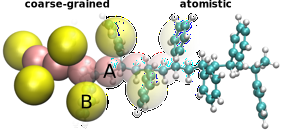
\includegraphics[width=0.5\textwidth]{./Figures/temporal_coherent_bm/intro.pdf}
  \caption{Illustration of the temporal coherent backmapping approach. Consecutive trajectory frames are spaced by time $\tau$. The ML model generates an atomistic frame $\mathbf{r}_t$ at time $t$ based on the previous atomistic state $\mathbf{r}_{t-\tau}$, the current coarse-grained frame $\mathbf{R}_{t}$ and latent sample $\mathbf{z}$ from a prior distribution $\mathcal{Z}$.}
  \label{FIG:TEMP_COH_intro}
\end{figure}


In this chapter, a new method to perform temporally coherent backmapping of molecular simulation trajectories is introduced. In particular, temporal coherent backmapping refers to reproducing shifts of atomic positions between consecutive frames that are comparable to the atomistic reference system. The proposed method aims at both, generating well-equilibrated molecular structures for each individual frame, while maintaining temporal coherence within a series of frames. To this end, a ML model is deployed that reconstructs a molecular structure leveraging configuration information from previous simulation frames. In particular, the model is conditioned on the current coarse- and previous fine-grained state (see Fig. \ref{FIG:TEMP_COH_intro}). In contrast to the previously deployed GAN-based method deepbackmap (DBM), a conditional variational autoencoder (CVAE) is used for this task. 

The method is applied to two biomolecular systems: Alanine dipeptide (ADP) and the mini protein chignolin (CLN). For each system two test sets are constructed: (1) An in-distribution test set is generated as a projection of all-atom (AA) trajectories onto the coarse-grained (CG) resolution. (2) A generalization test set is constructed by performing coarse-grained simulations deploying approximate force fields generated with CGSchNet, which is ML-based approach for molecular coarse-graining \cite{husic2020coarse}. The performance of the backmapping model is analyzed regarding its ability to reproduce structural, thermodynamic and dynamic properties of the reference system.

The work presented in this chapter stems from a collaboration with Kirill Shmilovich, Moritz Hoffmann and Nick Charron. The project originates from the long program \textit{Machine Learning for Physics and the Physics of Learning} at the Institute for Pure \& Applied Mathematics that was held from 09.04.19 to 12.08.19 at the University of California, Los Angeles. 

%The obtained trajectory is a set of states compatible with the starting condition, i.e. samples drawn from the accessible area in phase space.
\section{Method}

In the following, the proposed method is outlined. In addition, Markov state models are introduced as a framework to analyze dynamic properties of molecular systems.

\subsection{Backmapping Approach}

The proposed method is similar in spirit to the previously used method DBM (Sec. \ref{methology}), but differs in some aspects including the molecular representation, the incorporation of previous states and the architecture of the ML model. While this section emphasizes the distinctions to DBM, a detailed description of the applied ML model can be found in \cite{}(arXiv paper coming soon).

\subsubsection{Molecular Representation}

The ML model $g$ generates all atoms of a molecular snapshot in one step, i.e. not autoregressively. Therefore, the local environment representation used for DBM does not apply and molecular representations fed to the model have to capture the structure entirely. In particular, atoms and beads are represented as smooth densities expressed on a discretized grid due to voxelization. Note that the center of mass is removed for each molecule in order to ensure that it is fully enclosed by the grid representation. To avoid clutter, each particle is placed in its own feature channel, i.e. a molecule containing $N$ particles with positions $\mathbf{r} \in \mathbb{R}^{3N}$ is represented as a four-dimensional tensor $\mathcal{E}(\mathbf{r}) \in \mathbb{R}^{N \times s \times s \times s}$, where $s$ is the grid size. Note that $g$ also generates voxelized molecular representations $\hat{\mathcal{E}}$. However, these voxel representations can be transformed into Cartesian coordinates $\hat{\mathbf{r}} = m(\hat{\mathcal{E}})$, where $m$ denotes a sequence of differentiable operations. Further information on the voxel and coordinate representation can be found in Sec. \ref{DBM:representation}.

%$\gamma$ and $\Gamma$ (Eq. \ref{DBM:density_representation})
%Note that transforming these voxel representations can be transformed into Cartesian coordinates by a sequence of differentiable operations and therefore enables  within the computational graph of our model.

\subsubsection{Incorporating the Previous State}

Central to the proposed method is the incorporation of the previous state in order to achieve temporal coherence between trajectory frames. To this end, the input for the ML model $g$ at time $t$ is augmented with the previous atomistic state at time $t - \tau$, where $\tau$ is the lagtime between frames. In particular, the input for the generator $g$ consists of the current coarse-grained frame $\mathcal{E}(\mathbf{R}_{t})$ and previous atomistic frame $\mathcal{E}(\mathbf{r}_{t - \tau})$, where $\mathbf{R} \in \mathbb{R}^{3N}$ and $\mathbf{r} \in \mathbb{R}^{3n}$ denote the coordinates of the $N$ beads and $n$ atoms, respectively. While both, $\mathbf{R}_t$ and $\mathbf{r}_{t-\tau}$, are taken from the reference trajectory during training, atomistic coordinates $\mathbf{\hat{r}}_{t-\tau} = m\Big(g\big(\mathcal{E}(\mathbf{R}_{t - \tau}), \mathcal{E}(\mathbf{\hat{r}}_{t - 2\tau}) \big) \Big)$ generated by $g$ in the previous step are used during prediction. As such, trajectories are backmapped autoregressively. The seed for the hallucination, i.e. the initial atomistic frame at $t=0$, is selected from a presampled library of atomistic configurations based on the root-mean-square deviation at the coarse-grained resolution. 

\subsubsection{Variational Autoencoder}

A variational autoencoder (VAE) architecture (Sec. \ref{ML:explicit_models}) is used instead of the generative adversarial approach \cite{kingma2013auto}. To this end, an encoder network $e\big(\mathcal{E}(\mathbf{r}_{t})\big)$ is introduced to generate latent samples $\mathbf{\hat{z}}_{t} \in \mathbb{R}^d$ based on the current target frame $\mathbf{r}_{t}$, where $d$ is the dimension of the latent space. The decoder $g\big(\mathcal{E}(\mathbf{R}_{t}), \mathcal{E}(\mathbf{r}_{t - \tau}), \mathbf{\hat{z}}_t \big)$ is then trained to reconstruct the current state $\mathbf{r}_t$ given the low dimensional embedding $\mathbf{\hat{z}}_{t}$. As such, the model can be trained end-to-end based on a reconstruction loss and does not rely on an additional critic network.

While the encoder $e$ is indispensable during training, it is omitted at inference time. Instead, the latent sample $\mathbf{z}$ is drawn from a prior distribution in order to provide a source of randomness. This non-deterministic approach is an important aspect for the backmapping task, since each coarse-grained structure is associated with an ensemble of microstates. In particular, $\mathbf{z}$ is drawn from a 10-component Gaussian Mixture Model (GMM) fitted to the latent distribution implied by the encoder instead of the assumed prior $p(\mathbf{z}) \sim \mathcal{N}(\mathbf{0}, \mathbf{I})$. The GMM ensures that the decoder operates within densely sampled latent space regions \cite{ghosh2019variational}.

\subsubsection{Cost-function}

The cost-function $\mathcal{C}$ used to train the model end-to-end consists of multiple parts. In particular, a term $\mathcal{C}_{\text{recon vox}}$ is introduced to enforce reconstruction of the spatially voxelized particle densities, 

\begin{equation}
 \mathcal{C}_{\text{recon vox}}(\mathbf{r}_t, \hat{\mathcal{E}}) = \frac{1}{s^3n}\ || \mathcal{E}(\mathbf{r}_{t}) - \hat{\mathcal{E}} ||_2^2 .
\end{equation}

Similarly, a term $\mathcal{C}_{\text{recon pos}}$ is introduced to encourage the exact reconstruction of positions

\begin{equation}
 \mathcal{C}_{\text{recon pos}}(\mathbf{r}_t, \mathbf{\hat{r}}_t) = \frac{1}{3n}\ || \mathbf{r}_{t} - \mathbf{\hat{r}}_{t} ||_2^2 .
\end{equation}

In addition, the reproduction of inter-particle distances is targeted by a term $\mathcal{C}_{\text{EDM}}$ that computes the mean squared error between the Euclidean Distance Matrices (EDM) of the target configuration $\mathbf{r}$ and reconstructed configuration $\mathbf{\hat{r}}$,

\begin{equation}
  \mathcal{C}_{\text{EDM}}(\mathbf{r}_t, \mathbf{\hat{r}}_t) = \frac{1}{2n^2}\ || EDM(\mathbf{r}_{t}) - EDM(\mathbf{\hat{r}}_{t}) ||_2^2 .
\end{equation}

In order to achieve consistency between the backmapped structure $\mathbf{\hat{r}}$ and the given coarse-grained configuration $\mathbf{R}$, the coarse-grained mapping $M$ is applied to introduce a reconstruction loss $\mathcal{C}_{\text{CG}}$ at the coarse-grained resolution, i.e.

\begin{equation}
     \mathcal{C}_{\text{CG}}(\mathbf{R}_t, \mathbf{\hat{r}}_t) = \frac{1}{3N}\ || \mathbf{R}_t - M(\mathbf{\hat{r}}_t) ||_2^2  . \\
\end{equation}

Moreover, the atomistic force field is deployed in $\mathcal{C}_{\text{energy}}$ to calculate the mean squared error between the potential energies for the target structure $\mathbf{r}$ and reconstruction $\mathbf{\hat{r}}$,

\begin{equation}
  \mathcal{C}_{\text{energy}}(\mathbf{r}_t, \mathbf{\hat{r}}_t) = \lambda (U(\mathbf{{r}_{t}}) - U(\mathbf{\hat{r}}_{t}))^2 .
\end{equation}

This term serves as a regularizer to improve the quality of backmapped structures. It accelerates convergence and helps to match the reconstructed energetics to the ground truth trajectory. Since the potential energy is sensitive to small perturbations of the coordinates, it can become dominatingly large during early stages of training before the model learns to localize atomic coordinates. As a remedy, the prefactor $\lambda$ is incorporated, which is set to $\lambda = 0$ at the beginning of the training and slowly annealed up to $\lambda = 1$ using an exponential annealing schedule.

Finally, a regularization term $\mathcal{C}_{\text{KL}}$ is applied to bias the approximate posterior $\mathbf{\hat{z}} = e\big(\mathcal{E}(\mathbf{r})\big)$ towards the desired prior distribution, i.e. a normal distribution $\mathcal{N}(0,\mathbf{I})$ \cite{kingma2013auto},

\begin{equation}
 \mathcal{C}_{\text{KL}}(\mathbf{\hat{z}}) = \beta \mathcal{D}_{KL}(\mathbf{\hat{z}}||\mathcal{N}(0,\mathbf{I})).
\end{equation}

The associated prefactor $\beta$ scales the regularization loss and is set to $\beta = 1$ for the CLN model, while a cyclic annealing schedule is applied for ADP to mitigate KL vanishing \cite{fu2019cyclical}.

%(1) Molecules are considered in vacuum and not in the condensed-phase. As such, representations and the backmapping protocol can be simplified. 
\subsection{Markov State Model}
\label{TEMP_BM:MSM}

Central to the evaluation of the proposed method is the analysis of dynamic properties. To this end, Markov state models (MSM) are deployed to identify transitions between metastable states and their associated time scales \cite{husic2018markov, noe2019markov}. In particular, MSM is a framework to analysis time-series data, which is often used for MD trajectories. In its core, a MSM decomposes the configuration space into discrete and disjoint states, and describes the dynamics of the system by a transition matrix $\mathbf{P}$. The elements of the transition matrix $P_{ij}(\tau)$ denote the transition probability from state $i$ to state $j$ during the lagtime $\tau$. Note that a MSM model is a memoryless model, i.e. transitions only depend on the current state. Once the transition matrix $\mathbf{P}(\tau)$ is constructed from simulation data, the matrix can be decomposed into eigenvalues $\lambda_i$ and eigenvectors $\Psi_i$,

\begin{equation}
  \mathbf{P}(\tau) \Psi_i = \lambda_i \Psi_i .
\end{equation}

The largest eigenvalue is always $\lambda_1 =1$ and corresponds to the stationary distribution. Subsequent eigenvalues $\lambda_{i>1}$ are associated with characteristic timescales, also called implied timescales, of dynamic processes described by the eigenvectors $\Psi_{i>1}$.

\section{Set-up and Reference Data}

The proposed method is applied to the backmapping of two biomolecular systems: Alanine dipeptide (ADP) and the mini protein chignolin (CLN). Illustrations of both molecules at the atomistic and coarse-grained level can be found in Fig. \ref{FIG:TCBM_molecules}. Data sets for training and testing of the model consist of pairs of corresponding atomistic and coarse-grained trajectories, which are obtained by mapping atomistic trajectories onto the coarse-grained representation. Since the test set is obtained similarly to the training set, it will be referred to as in-distribution test set in the following. Moreover, a generalization test set is constructed that consists of coarse-grained trajectories obtained with a MD simulation performed at the coarse-grained resolution. To this end, a coarse-grained force field is deployed that has been generated by CGSchNet, which is a ML-based method for force field parameterization \cite{wang2019machine, husic2020coarse}.

\begin{figure}[H]
  \centering
      \includegraphics[width=1.0\textwidth]{./Figures/temporal_coherent_bm/representation.pdf}
  \caption{Atomistic (left) and coarse-grained (right) representations of (a) alanine dipeptide and (b) chignolin.}
  \label{FIG:TCBM_molecules}
\end{figure}

\subsection{ADP}

Alanine dipeptide mimics the dynamics of the amino acid alanine in a peptide chain and has been used as a model system in numerous previous studies \cite{smith1999alanine, vitalini2015dynamic, nuske2014variational, nuske2017markov}.

MD simulations to obtain atomistic trajectories for ADP are performed in explicit water. Simulations are carried out in the microcanonical (NVE) ensemble using the molecular dynamics package OpenMM \cite{eastman2017openmm}. In particular, the AMBER ff-99SB-ILDN force field is deployed and a cubic box containing 651 TIP3P water molecules randomly placed within a volume of (2.7273~nm)$^3$ is used \cite{lindorff2010improved}. The length of all bonds involving hydrogen atoms are constrained. A time step of $2.0$ fs is used and initial velocities are sampled from a Maxwell-Boltzmann distribution at $300$ K. During production, snapshots are recorded every $1.0$ ps. The training set comprises $500 000$ and the test set $250 000$ frames, respectively.

The 22 atoms of ADP are coarse-grained into 6 beads. More specifically, the coarse-grained representation for ADP consists of 5 backbone carbon and nitrogen atoms (C, N, CA, C, N) and the carbon beta (CB) of the alanine residue. Water molecules are treated implicitly, i.e. water is removed from the representation. Coarse-grained forces obtained from the atomistic simulations are used for the training of CGSchNet and the training routine follows the procedure in \cite{husic2020coarse}. The force field produced by CGSchNet is deployed to generate generalization data. The MD settings for the coarse-grained simulation are equivalent to the settings used for the atomistic simulation, except for a increased integration timestep of $4.0$ fs. Snapshots are recorded every $1.0$ ps and a total of $400 000$ samples are collected.

%Electrostatics were treated deploying the particle-mesh Ewald (PME) method using a $1.0$ nm cutoff for the direct space interactions.


\subsection{CLN}

The proposed method is also tested on a much more challenging data set of the mini protein chignolin (CLN), which is composed of 10 amino acids plus termini. CLN displays a clear folding/unfolding transition when solved in water \cite{satoh2006folding}.

Reference atomistic trajectories for CLN are provided by Wang \emph{et al.} and are already reported in \cite{wang2019machine}. In particular, MD simulations are performed using the MD software ACEMD \cite{harvey2009acemd} deploying the CHARMM22$^{*}$ \cite{piana2011robust} force field and the TIP3P \cite{jorgensen1983comparison} water model. Simulations are carried out in the $NVT$ ensemble at $350$ K. Adaptive sampling is used to sufficiently sample folding/unfolding transitions of CLN facilitated by a Markov State Model \cite{prinz2011markov}. $3 744$ separate trajectories of $50$ ns are recorded aggregating a total simulation time of $\sim 187$ $\mu$s. Within each trajectory samples are spaced by $100$ ps. The training set comprises $3 650$ and the test set $94$ independent trajectories. For additional details regarding the CLN simulations the reader is referred to the work of Wang \emph{et al.}\cite{wang2019machine}.

While CLN consists of 175 atoms, it is coarse-grained into 10 beads. In particular, the coarse-grained representation for CLN consists of the 10 sequential $\alpha$-carbons along the molecular backbone. Generalization data is generated by coarse-grained simulations performed with OpenMM in the $NVT$ ensemble at $350$ K. $1000$ independent trajectories are generated starting from random configurations mapped from the atomistic trajectories. Each coarse-grained trajectory consists of $4000$ frames spaced by $100$ ps.

\section{Results}

The performance of the trained model is evaluated in terms of its capability to reproduce energetic, thermodynamic and dynamic properties of the AA reference system. The model is used to backmapped in-distribution as well as generalization data. Note that the generalization data represents a more difficult backmapping exercise, as the model has to generalize to unseen simulated data generated by a different, approximate force field than the model was trained on.

\subsection{Energetics}

The potential energy distributions displayed in Fig. \ref{FIG:TCBM_energies} serve as an indicator for the overall structural similarity between AA reference and backmapped structures. The energy distributions obtained for ADP shown in panel (a) reveal that the ML model is able to reproduce energetic properties with remarkable accuracy. While small high-energy tails can be observed for reconstructed molecules, the overall agreement of both test sets with the reference system is excellent. 

Turning to the energy distributions for the more challenging mini protein CLN in panel (b) indicates a similar performance. However, the model supresses structures with low energies compared to the reference system. Moreover, a discrepancy between the distributions obtained for the in-distribution and generalization test sets can be observed. In particular, the energy distribution for the generalization set displays a tail towards high energies that is not observed in the in-distribution test set.

\begin{figure}[H]
  \centering
      \includegraphics[width=1.0\textwidth]{./Figures/temporal_coherent_bm/energies.pdf}
  \caption{Distributions of the potential energy obtained for the reference system, backmapped in-distribution test set and backmapped generalization test set for (a) alanine dipeptide and (b) chignolin.}
  \label{FIG:TCBM_energies}
\end{figure}

\subsection{Thermodynamics}

In order to test thermodynamic agreement between the reference system and the backmapped test sets, free energy surfaces (FES) are constructed. The FES are generated in the space of collective variables $\mathbf{q}$, i.e. low-dimensional variables that characterize the configurational state of the system. More specifically, relative populations $N(\mathbf{q}_i)$ are computed for discretized states $\mathbf{q}_i$ yielding free energies $F(\mathbf{q}_i) = - k_{\text{B}}T \text{ln}(N(\mathbf{q)_i)} + \text{const}$. To faithfully represent free energies, population histograms are MSM reweighted to account for finite sampling effects and bias induced by the initialization of the simulation. %The MSM is constructed as explained in Sec. \ref{TEMP_BM:MSM}.

The FES and selected snapshots for ADP can be found in Fig. \ref{FIG:TCBM_free_energy_adp}. The FES are computed in terms of the backbone dihedrals $\phi$ and $\psi$, as they are well known collective variables to describe the conformational states of ADP \cite{nuske2014variational,vitalini2015dynamic}. Panel (a) displays the FES obtained for the reference data. Three characteristic metastable states are observed that correspond to $\beta$-sheet (snapshots 1 and 2), $\alpha$-helix (snapshot 3), and left-handed $\alpha$-helix (snapshots 4 and 5) conformations of the amino acid. The atomistic reconstruction for the in-distribution test set can be found in panel (b). The model accurately reproduces all metastable states and is visually in excellent agreement with the reference FES. Similarly, the FES obtained for the backmapped generalization test set matches remarkable well with the reference FES, as shown in panel (c). However, some regions along transition paths between metastable states display higher relative populations compared to the reference system, for example ($\phi\approx-2$,$\psi\approx-2$). While the coarse-grained force field enables broader and more frequent exploration of these regions of configuration space, they are under represented in the atomistic trajectory. Therefore, it is remarkable that the ML model generalizes to those sparsely sampled areas and reconstructs high-energy configurations accordingly. The structural fidelity of reconstructed configurations is further highlighted by superimposed collections of snapshots displayed in panel (d). Note that backmapped structures of a superposition are sampled using a fixed CG structure but varying latent samples $\mathbf{z}$. As such, the superpositions emphasize the non-deterministic aspect of this backmapping prodcedure. For both test sets, the ML model reconstructs visually faithful configurations with remarkable similarity to the atomistic reference data.

\begin{figure}[H]
  \centering
      \includegraphics[width=1.0\textwidth]{./Figures/temporal_coherent_bm/ADP_fes.pdf}
  \caption{Comparison of atomistic and backmapped MSM-reweighted free energy surfaces (FES) for ADP computed in terms of the backbone dihedrals $\Phi$ and $\Psi$. Ramanchandran plots are shown for (a) the atomistic reference in-distribution test set, (b) backmapped in-distribution test set and (c) backmapped generalization test set. Labels in (a) denote locations for the five metastable states of ADP. Panel (d) displays superimposed configurations for each metastable state}
  \label{FIG:TCBM_free_energy_adp}
\end{figure}

Fig. \ref{FIG:TCBM_free_energy_cln} displays the FES and selected snapshots obtained for CLN. Unlike ADP, constructing meaningful collective variables for CLN is more challenging. To this end, time-lagged independent component analysis (TICA) is used for dimensionality reduction, as outlined in Sec. \ref{MS:sketchmap}. The TICA algorithm is applied to the atomistic reference data to obtain a low dimensional projection of the 45 pairwise $\alpha$-carbon distances. In particular, the first two non-trivial independent components (ICs) are used as collective variables in the following. The FES obtained for the reference data is displayed in panel (a). Three metastable states can be identified that correspond to the folded state (snapshot 1), mis-folded state (snapshot 2) and folded state (snapshot 3). While all metastable states can be recovered upon backmapping of the in-distribution and generalization test sets (panel (b) and (c)), the FES for backmapped trajectories are contracted compared to the reference FES. In particular, the diversity of folded and mis-folded states is reduced upon backmapping compared to the reference system. This is also indicated by a lower variability of backmapped structures for the folded and mis-folded states displayed in panel (d). Similarly to ADP, backmapping of the generalization test set yields higher populations along the transition paths between metastable states compared to the in-distribution test set. 

\begin{figure}[H]
  \centering
      \includegraphics[width=1.0\textwidth]{./Figures/temporal_coherent_bm/CLN_fes.pdf}
  \caption{Comparison of atomistic and backmapped MSM-reweighted free energy surfaces (FES) for CLN computed in terms of the first two non-trivial independent components obtained by time-lagged independent component analysis for the 45 pairwise $\alpha$-carbon distances. Ramanchandran plots are shown for (a) the atomistic reference in-distribution test set, (b) backmapped in-distribution test set and (c) backmapped generalization test set. Labels in (a) denote locations for the three metastable states of CLN. Panel (d) displays superimposed configurations for each metastable state}
  \label{FIG:TCBM_free_energy_cln}
\end{figure}

%While transition paths between metastable states are less populated in the backmapped in-distribution test set compared to the reference data, the discrepancy between the total number of data points between both data sets has to be emphasized.

\subsection{Dynamics}

A key feature of the proposed method is the incorporation of the previous trajectory frame as a conditional input for the ML model. Such temporal information is required to achieve temporal coherence between consecutive frames and sets the method apart from other backmapping schemes. In this section, kinetic properties of backmapped trajectories are analysed in terms of implied timescales of slow processes obtained with MSMs. In addition, temporal coherence between frames is tested in terms of intra-frame velocities.

\subsubsection{Timescales of Slow Processes}

MSM are constructed as outlined in Sec. \ref{TEMP_BM:MSM} deploying the collective variables used previously for the analysis of thermodynamic properties. In particular, the space of collective variables is decomposed using k-means clustering. For a direct comparison between timescales and processes between different MSMs, the same cluster centers obtained for the atomistic reference data are deployed for all data sets. To evaluate the similarity between processes, the cosine similarity $c$ between two eigenvectors $\mathbf{\Psi}_i$ and $\mathbf{\Psi}_j$ is computed as 

\begin{equation}
 c = \frac{\mathbf{\Psi}_i \mathbf{\Psi}_j}{|\mathbf{\Psi}_i| |\mathbf{\Psi}_j|} .
\end{equation}

Moreover, collective variables for both systems can be computed at the coarse-grained resolution as well allowing for MSM construction of coarse-grained trajectories. Note that coarse-grained force fields typically yield faster simulation dynamics compared to atomistic force fields. To facilitate comparison between all trajectories, implied timescales obtained for coarse-grained simulation data are rescaled such that the timescales for the slowest process match.

Fig. \ref{FIG:TCBM_kinetics_adp} displays the implied timescales obtained for ADP trajectories. MSMs are build for a lagtime of 5 ps and 100 cluster centers are used for the state decomposition. For all data sets a cosine similarity  $>90$ \% to the reference system is observed for the first three processes. A comparison for the implied timescales between atomistic reference and reconstructed in-distribution trajectories can be found in panel (a). The first three timescales are in excellent agreement and match within error. Note that subsequent timescales are below the resolution limit of the MSMs, since corresponding processes are faster than the applied lagtime. Implied timescales for the first three processes obtained for the backmapped generalization set displayed in panel (b) also match remarkable well with the reference system. Moreover, timescales obtained for the backmapped generalization set and coarse-grained trajectories prior to backmapping are in excellent agreement. This indicates that the ML model maintains the kinetics of slow motions present in the coarse-grained trajectories. 

\begin{figure}[H]
  \centering
      \includegraphics[width=1.0\textwidth]{./Figures/temporal_coherent_bm/ADP_kinetics.pdf}
  \caption{Comparison of implied timescales for ADP obtained by a MSM constructed in terms of the backbone dihedrals $\Phi$ and $\Psi$. Timescales are shown for (a) the atomistic reference in-distribution test set and backmapped in-distribution test set, as well as (b) the atomistic reference in-distribution test set, backmapped generalization test set and coarse-grained generalization test set.}
  \label{FIG:TCBM_kinetics_adp}
\end{figure}


A similar analysis for the timescales of slow processes obtained for CLN can be found in Fig. \ref{FIG:TCBM_kinetics_cln}. The implied timescales obtained for the atomistic reference system are reproduced within error upon backmapping of the in-distribution test set, as can be seen in panel (a). However, a cosine similarity $>90$ \% is only observed for the first two processes, while the third process yields $\approx 80$ \% and the fourth process $\approx 60$ \% similarity. This indicates that the third and fourth slowest processes have slightly changed upon backmapping. Turning to the timescales obtained for the CGSchNet coarse-grained simulation in panel (b) reveals that timescales of different processes are not rescaled uniformly when the coarse-grained force field is deployed. While timescale ratios of the 1st, 3rd and 4th process are consistent with the kinetics observed for the atomistic reference system, the second process is accelerated more than the others. However, cosine similarities of the first and second process is $\approx 60$ \%, while a similarity $<25$ \% for the third and fourth process is observed. As such, timescales comparisons are not reliable for the third and subsequent processes. Backmapping the coarse-grained trajectory yields similar timescales compared to the coarse-grained kinetics for the first and second process, while the third and fourth process are slowed down. 

In conclusion, the backmapped trajectories reflect the slow dynamics of the underlying coarse-grained trajectories.

\begin{figure}[H]
  \centering
      \includegraphics[width=1.0\textwidth]{./Figures/temporal_coherent_bm/CLN_kinetics.pdf}
  \caption{Comparison of implied timescales for CLN obtained by a MSM constructed in terms of the first two independent compoenents of the time-lagged independent component analysis for the 45 pairwise $\alpha$-carbon distances. Timescales are shown for (a) the atomistic reference in-distribution test set and backmapped in-distribution test set, as well as (b) the atomistic reference in-distribution test set, backmapped generalization test set and coarse-grained generalization test set.}
  \label{FIG:TCBM_kinetics_cln}
\end{figure}

%In conclusion, the backmapped trajectories reflect the slow dynamics of the underlying coarse-grained trajectories.
%The cosine similarity of the second process is improved to $\approx 90$ \% upon backmapping, while the similarities of other processes are maintained.
\subsubsection{Intra-frame Velocities}

As a measure for temporal coherence, the shift of atomic positions between consecutive frames is analyzed, i.e. the intra-frame velocities. In particular, atomic velocities $\mathbf{v}_i$ for a frame at time $t$ are calculated as the deviations of atomic positions $\mathbf{s}_i$ between consecutive frames,

\begin{equation}
  \mathbf{v}_i(t) = \frac{\mathbf{s}_i(t) - \mathbf{s}_i(t - \tau)}{\tau} ,
\end{equation}

where $\tau$ is the lagtime between frames. Fig. \ref{FIG:TCBM_velocities} displays the intra-frame velocity distributions obtained for the reference trajectory and both reconstructed test sets. In addition, intra-frame velocity distributions obtained for a baseline backmapping method are shown. The baseline method is fragment-based and treats each frame separately. More specifically, a library consisting of 40000 pairs of equilibrated atomistic and associated coarse-grained frames is generated for both systems. Backmapping of a coarse-grained frame is performed by selecting the closest matching coarse-grained structure from the library in terms of root-mean-square deviation and projecting the corresponding atomistic structure onto the coarse-grained representation. 

The velocity distributions for ADP can be found in panel (a). The backmapped distribution obtained for the in-distribution test set deploying the proposed temporal coherent backmapping scheme is in excellent agreement with the reference distribution. On the other hand, the frame-based baseline method yields a velocity distribution for the in-distribution test set that differs from the reference system and is slightly shifted to higher velocities. Backmapping of the generalization set deploying the ML model yields significantly higher intra-frame velocities, which is reasonable as this reflects the acceleration of the coarse-grained dynamics.

The results obtained for CLN are displayed in panel (b). Temporal coherent backmapping yields a velocity distribution for the in-distribution test set that matches remarkably well with the reference distribution. Similarly to ADP, the baseline method is not able to reproduce the reference velocities. Moreover, velocities obtained for the generalization set deploying the ML model are significantly higher compared to the reference system.

\begin{figure}[H]
  \centering
      \includegraphics[width=1.0\textwidth]{./Figures/temporal_coherent_bm/velocities.pdf}
  \caption{Comparison of the intra-frame velocity distributions for (a) alanine dipeptide and (b) chignolin as a measure for temporal coherence. Distributions are computed for the atomistic reference, backmapped in-distribution test set and backmapped generalization test set. In addition, a frame-based baseline method is applied to the in-distribution test set.}
  \label{FIG:TCBM_velocities}
\end{figure}

%Temporal coherence of backmapped trajectories is tested in this section in terms of implied process timescales and velocity distributions.
\section{Discussion}

In this chapter, a new ML-based method for temporal coherent backmapping of molecular trajectories is introduced. In particular, a conditional variational autoencoder (cVAE) is trained to non-deterministically reinsert atomistic details conditioned on the current coarse-grained and the previous atomistic frame. 

The approach is applied to two popular biomolecular systems: Alanine dipeptide (ADP) and the miniprotein chignolin (CLN). The performance of the ML model is analyzed regarding its ability to reproduce structural, thermodynamic and dynamic properties of the reference system. To this end, the method is applied to an in-distribution test set that consists of atomistic structures projected onto the coarse-grained resolution. Excellent structural similarity between the reference system and the backmapped in-distribution test set is observed evaluated in terms of potential energy distributions. Moreover, thermodynamic properties match remarkably well, which is tested by analyzing free energy surfaces that are constructed in terms of collective variables. In order to analyze dynamic properties, MSMs are constructed in the space of collective variables to identify slow processes and their associated timescales. The obtained timescales of the backmapped trajectory agree remarkably well with the dynamics observed for the atomistic reference system. Temporal coherence between consecutive frames is evaluated in terms of intra-frame velocity distributions, which are reproduced with excellent accuracy deploying the ML model. The benefit of incorporating the previous state of the system as an additional input is highlighted by a comparison against a frame-based baseline method, which yields velocity distributions that differ significantly from the reference.  

In addition, backmapping of a generalization test set is performed, which consists of trajectories obtained in a coarse-grained simulation based on approximate force fields generated by CGSchNet. While structural and thermodynamic properties of the reference system are reproduced with remarkable accuracy upon backmapping of this generalization data, dynamic properties differ. Timescale ratios of slow transitions between metastable states are recovered for ADP, but deviate from the atomistic reference for CLN. Moreover, intra-frame velocities of the backmapped generalization trajectories are significantly higher compared to the reference. However, a difference of dynamic properties is expected for this test set: Coarse-grained simulations typically display faster dynamics compared to atomistic simulations as a direct consequence of deploying a reduced representation. Averaging over degrees of freedom effectively smoothens the energy landscape allowing for a faster exploration of phase space. However, timescales for transitions between metastable states are typically not rescaled uniformly yielding timescale ratios that differ from the atomistic reference system \cite{fritz2011multiscale}. As such, backmapped trajectories reflect the kinetics of the underlying coarse-grained trajectories.

Moreover, the cVAE approach non-deterministically reinserts atomistic details along the coarse-grained variables. This feature is highlighted by a visual inspection of backmapped structures sampled from a fixed coarse-grained structure but differing latent samples. This procedure yields an ensemble of atomistic microstates that are all consistent with the given coarse-grained structure but still display variations.

In summary, the proposed method is able to backmap coarse-grained trajectories such that (1) each reconstructed frame has a high statistical weight, (2) each frame is a valid reconstruction of the given coarse-grained structure, i.e. atomistic degrees of freedom are reinserted along the coarse-grained variables and (3) consecutive frames are temporally coherent, i.e. shifts in atomic positions between consecutive frames follow the same distribution as the atomistic reference system. As such, the proposed method offers the ability to analyze the dynamics of a coarse-grained simulation at atomistic resolution.

Future work might focus on different strategies to improve the training protocol of the approach: (1) In order to improve sampling of configuration space, training samples of sparsely populated regions in configuration space can be emphasized more. This could be realized by accompanying training samples with thermodynamic or dynamical path weights. (2) An autoregressive training protocol could be applied to improve the temporal coherence. In particular, a recurrent neural network approach could add information of multiple consecutive frames to the gradients used during backpropagation. (3) To further encourage the ML model to utilize knowledge of previous states for its predictions, the training loss could be augmented with a reconstruction error of properties that are explicitly based on such information, for example intra-frame velocities. 

